\documentclass[a4paper, 12pt]{article}
\usepackage[utf8]{inputenc}
\usepackage{natbib}
\usepackage{graphicx}
\usepackage{algorithm2e}
\usepackage{listings}
\usepackage{hyperref}

\title{OOP Homework 2 - Problem 11}
\author{Vasilescu Vlad}
\date{Documentation}

\begin{document}

\maketitle

\section*{Overview}
The Petri Net is formed by transitions and places which replace the vertices in a normal graph and arcs which connect the
places to the transitions. A place can only be connected to a tranisiton and vice versa.
All arcs are weighted and places may contain a number of tokens. Each place may have a name.\\
A transition is "enabled" if the places connected to the left contain at least as many tokens as the weight on the arc.
If a transition is enabled it can be "fired", thus removing a number of tokens equal the weight on the arc from each previous place
and placing them in the following places.

\section*{Petri net methods:}
Here is an overview of the functions used by the petri net:

\subsection*{Checking if a transiton is enabled:}
We assume the transition is enabled and check for otherwise.

\begin{algorithm}[H]
    \KwData{Transition ID}
    \KwResult{A boolean value}
    transition is enabled\;
    \ForAll{input places}{
        \If{place's condition is not satisfied}{
            transition is not enbaled\;
        }
    }
    return transition state\;
    
    \caption{Transition state check}
\end{algorithm}

\subsection*{Firing a transition}
We first check if the transition we wish to fire is enabled and then proceedes with the algorithm described.

\begin{algorithm}[H]
    \KwData{Transition ID}
    \KwResult{Transition is fired}
    \ForAll{input places} {
        remove tokens equal the the connecting arc's weight from each\;
    }
    \ForAll{output places} {
        place tokens equal to the ammount removed\;
    }
    \caption{Transition firing}
\end{algorithm}
    
\subsection*{Output current state}
We iterate trough each place and print the place's name and the ammount of tokens it currently contains.

\begin{algorithm}[H]
    \KwResult{Place info for each place}
    \ForAll{places}{
        print place's name and no. of tokens\;
    }
    \caption{Finding a contact.}
\end{algorithm}

\section*{Helper methods:}

\subsection*{Creating the Petri Net from a ".np" file:}
We parse the file formatted in the following way:

\begin{lstlisting}[basicstyle=\footnotesize]
no_places no_trans
p[0].name p[1].name ... p[no_places].name
p[0].no_tokens p[1].no_tokens ... p[no_places].no_tokens
no_inputs no_outputs
t[0].input[0].dest t[0].input[0].weight
...
t[0].input[no_inputs].dest t[0].input[no_inputs].weight
t[0].output[0].dest t[0].output[0].weight
...
t[0].output[no_outputs].dest t[0].output[no_outputs].weight
...
...
...
no_inputs no_outputs
t[no_trans].input[0].dest t[no_trans].input[0].weight
...
t[no_trans].input[no_inputs].dest t[no_trans].input[no_inputs].weight
t[no_trans].output[0].dest t[no_trans].output[0].weight
...
t[no_trans].output[no_outputs].dest t[no_trans].output[no_outputs].weight
\end{lstlisting}
and create a Petri Net from it.

\subsection*{Creating a ".np" file from user input.}
We create a file in the format specified above from the instructions given.

\section*{Example net:}
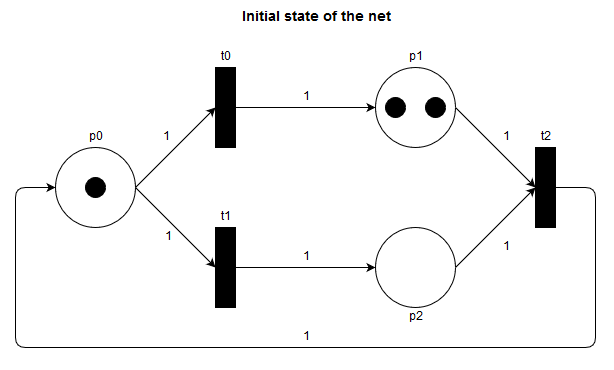
\includegraphics[scale=0.8]{init_state.png}

\subsection*{State of net before firing any transition:}
\begin{lstlisting}
Tokens in p0: 1
Tokens in p1: 2
Tokens in p2: 0
\end{lstlisting}

\subsection*{State of the net after firing transition 1:}
\begin{lstlisting}
Fired transition 1.

Tokens in p0: 0
Tokens in p1: 2
Tokens in p2: 1
\end{lstlisting}

\subsection*{State of the net after firing transition 1 and 2:}
\begin{lstlisting}
Fired transition 2.

Tokens in p0: 1
Tokens in p1: 1
Tokens in p2: 0
\end{lstlisting}

\section*{Links:}
\href{https://en.wikipedia.org/wiki/Petri_net}{Petri Net - Wikipedia}\\
\href{https://github.com/metwadsprite/OOP-Homework-2}{GitHub Repository}

\end{document}
